% Historical biographies: original summaries, with linked institutional sources.
% Portrait provenance and reuse limits: chapter-figures/portraits.md.
% Portraits lacking explicit reuse terms carry individual permission-pending notices.

\newcommand{\hfBioHartree}{%
\hfbiography{Douglas Rayner Hartree (1897--1958)}
{\hfbiophoto{chapter-figures/portrait-hartree.jpg}}
{An English mathematician and physicist, Hartree worked at Manchester before
returning to Cambridge as Plummer Professor of Mathematical Physics in 1946.
His 1928 self-consistent-field method made atomic structure accessible through
iterative numerical solutions of one-electron equations \citep{Hartree1928}.
He also helped develop mechanical and electronic computing: for Hartree,
theoretical approximations and the means of actually solving their equations
were inseparable concerns.}
{Biography: \href{https://mathshistory.st-andrews.ac.uk/Biographies/Hartree/}{University of St Andrews, MacTutor}.
Portrait: unknown photographer, c.~1940;
\href{https://commons.wikimedia.org/wiki/File:Douglas_hartree.jpg}{Centre for Computing History / Wikimedia Commons}, listed as public domain.}}

\newcommand{\hfBioWilliamHartree}{%
\hfbiography{William Hartree (1870--1943)}
{\hfbiophoto{chapter-figures/portrait-william-hartree.jpg}}
{An English engineer and numerical researcher, William Hartree taught at
Cambridge and later collaborated with the physiologist A.~V.~Hill. He was
Douglas Hartree's father and an important collaborator in turning atomic
self-consistent-field theory into numerical results. Their joint 1935
beryllium study included exchange explicitly \citep{HartreeHartree1935}.
His contribution illustrates a less visible part of the method's history:
obtaining accurate atomic orbitals required sustained numerical work as
well as the formulation of the equations.}
{Biography: \href{https://doi.org/10.1038/152154a0}{A.~V.~Hill, Nature obituary, 1943};
\href{https://mathshistory.st-andrews.ac.uk/Biographies/Hartree/}{MacTutor Hartree biography}.
Photograph: \href{https://sliderulemuseum.org/Yearbooks.shtml}{International Slide Rule Museum archive}, late 1930s;
photographer unspecified. \textbf{Draft reproduction: permission pending.}}}

\newcommand{\hfBioSwirles}{%
\hfbiography{Bertha Swirles, Lady Jeffreys (1903--1999)}
{\hfbiophoto{chapter-figures/portrait-swirles-source.pdf}}
{A British mathematician trained at Girton College, Cambridge, Swirles
worked on quantum theory before returning to Girton as a Fellow in 1938.
Her 1935 relativistic self-consistent-field treatment extended the atomic
orbital framework beyond the non-relativistic approximation
\citep{Swirles1935}. With Douglas and William Hartree, she also studied
exchange and the superposition of configurations in a 1939 paper on oxygen
\citep{HartreeHartreeSwirles1939}. These were distinct extensions of the
ordinary single-determinant theory developed here. Her subsequent teaching
and the book \emph{Methods of Mathematical Physics}, written with Harold
Jeffreys, influenced generations of mathematical physicists.}
{Biography: \href{https://mathshistory.st-andrews.ac.uk/Biographies/Jeffreys_Bertha/}{University of St Andrews, MacTutor}.
Portrait: Dr John Davies, \href{https://www.girton.cam.ac.uk/sites/default/files/2020-10/CoB10YearBooklet.pdf}{Girton College, Celebrating Our Benefactors booklet, 2017 entry}; photograph date unspecified.
\textbf{Draft reproduction: permission pending.}}}

\newcommand{\hfBioDirac}{%
\hfbiography{Paul Adrien Maurice Dirac (1902--1984)}
{\hfbiophoto{chapter-figures/portrait-dirac.jpg}}
{Born in Bristol, Dirac trained in engineering and mathematics before
becoming one of the founders of quantum mechanics at Cambridge. His 1930
paper on exchange expressed the exchange-corrected self-consistent-field
theory in terms of a one-particle density matrix and explicitly examined
invariance under changes of occupied orbitals \citep{Dirac1930}. This
formulation makes the occupied subspace, rather than a particular set of
orbitals spanning it, the central object. It is distinct from the local
exchange approximation for the Thomas atom also developed in that paper.}
{Biography: \href{https://mathshistory.st-andrews.ac.uk/Biographies/Dirac/}{University of St Andrews, MacTutor}.
Portrait: Nobel Foundation, 1933,
\href{https://commons.wikimedia.org/wiki/File:Paul_Dirac,_1933.jpg}{via Wikimedia Commons, listed as public domain}.}}

\newcommand{\hfBioMcWeeny}{%
\hfbiography{Roy McWeeny (1924--2021)}
{\hfbiophoto{chapter-figures/portrait-mcweeny.jpg}}
{A British theoretical chemist, McWeeny earned his doctorate with Charles
Coulson at Oxford and worked in Newcastle, Keele, and Sheffield before
moving to Pisa in 1982. His work made reduced density matrices a powerful
language for electronic structure. His 1960 account \citep{McWeeny1960}
brought together their use in orbital theories, connecting electron
densities, energies, and the constraints associated with a determinantal
state. His wider contributions included valence-bond theory,
multiconfigurational SCF methods, and the response of molecules to external
fields.}
{Biography: \href{https://www.iaqms.org/obituary/McWeenyObituary.pdf}{Brian Sutcliffe and Michael Robb, IAQMS obituary, 2021}.
Portrait: \href{https://www.iaqms.org/deceased/mcweeny.php}{IAQMS archive}; photographer and date unspecified.
\textbf{Draft reproduction: permission pending.}}}

\newcommand{\hfBioPaldus}{%
\hfbiography{Josef Paldus (1935--2023)}
{\hfbiophoto{chapter-figures/portrait-paldus.jpg}}
{A Czech-born Canadian theoretical chemist, Paldus trained in Prague and
joined the University of Waterloo in 1968. With Ji\v{r}\'{i}
\v{C}\'{i}\v{z}ek, he developed the analysis of Hartree--Fock stability,
including the distinction between singlet and triplet instabilities in
closed-shell systems \citep{CizekPaldus1967}. This work clarified why a
self-consistent solution need not be an energy minimum. Their collaboration
also helped establish coupled-cluster theory in molecular quantum chemistry.
Paldus developed unitary-group methods for treating spin-adapted
many-electron states \citep{Paldus1974}, bringing algebraic structure to
configuration-interaction calculations. His later account with Jason
Stuber \citep{StuberPaldus2003} places the symmetry-broken determinants
discussed here in a systematic framework. His work thus connects the
classification of independent-particle states with the treatment of
electron correlation beyond a single determinant.}
{Biography: \href{https://uwaterloo.ca/applied-mathematics/news/memoriam-josef-paldus}{University of Waterloo, 2023 obituary};
\href{https://www.iaqms.org/deceased/paldus.php}{IAQMS profile}.
Portrait: IAQMS archive; photographer and date unspecified.
\textbf{Draft reproduction: permission pending.}}}

\newcommand{\hfBioBernardi}{%
\hfbiography{Fernando Bernardi}{}
{An Italian theoretical organic chemist at the University of Bologna,
Bernardi studied with Boys in Cambridge in 1969--1971. Their joint 1970
paper introduced the counterpoise procedure discussed here
\citep{BoysBernardi1970}, making the comparison of fragment basis spaces an
explicit part of intermolecular-energy calculations. His later research
connected electronic-structure methods with organic reactivity and
photochemistry, including work with Massimo Olivucci and Michael Robb on
potential-energy-surface crossings. The Boys--Bernardi name acknowledges
both contributors to a correction that remains central to the practical
use of atom-centered basis sets.}
{Biography: author profile in \href{https://doi.org/10.1039/CS9962500321}{Bernardi, Olivucci, and Robb, Chemical Society Reviews, 1996, p.~321}.
An authenticated portrait has not yet been included; the published source image was inaccessible.}}

\newcommand{\hfBioFock}{%
\hfbiography{Vladimir Aleksandrovich Fock (1898--1974)}
{\hfbiophoto{chapter-figures/portrait-fock.jpg}}
{Fock was a Russian theoretical physicist whose career was closely associated
with the university in his native St Petersburg, later called Leningrad.
In 1930 he incorporated exchange into the self-consistent-field equations by
using an antisymmetric many-electron wavefunction \citep{Fock1930}.
His work ranged from wave mechanics and gravitation to quantum field theory;
the Fock-space construction carries his name as well.}
{Biography: \href{https://www.iaqms.org/deceased/fock.php}{International Academy of Quantum Molecular Science (IAQMS)} and
\href{https://mathshistory.st-andrews.ac.uk/Biographies/Fock/}{MacTutor}.
Portrait: \href{https://www.iaqms.org/deceased/fock.php}{IAQMS archive}; photographer and date unspecified.
\textbf{Draft reproduction: permission pending.}}}

\newcommand{\hfBioBornOppenheimer}{%
\hfbiography{Born and Oppenheimer}{}
{\hfbioperson{Max Born (1882--1970)}{chapter-figures/portrait-born.jpg}
{A German-born physicist, Born helped establish quantum mechanics at
G\"ottingen and later taught at Edinburgh. His statistical interpretation of
the wavefunction brought him a share of the 1954 Nobel Prize in Physics.
His work with Oppenheimer addressed a different foundational question:
how to organize the electronic and nuclear motions of a molecule.}
\smallskip
\hfbioperson{J.~Robert Oppenheimer (1904--1967)}{chapter-figures/portrait-oppenheimer.jpg}
{The American theoretical physicist completed his doctorate at G\"ottingen
in 1927, the year of their joint molecular paper \citep{BornOppenheimer1927}.
He later taught at Berkeley and Caltech and directed the Institute for
Advanced Study. The approximation bearing their names supplies the
electronic-structure framework used here; it is distinct from the subsequent
Hartree--Fock approximation.}}
{Biographies: \href{https://www.nobelprize.org/prizes/physics/1954/born/facts/}{Nobel Foundation};
\href{https://www.ias.edu/oppenheimer-legacy}{Institute for Advanced Study}.
Portraits: Born, unknown photographer, \href{https://commons.wikimedia.org/wiki/File:Max_Born.jpg}{via Wikimedia Commons, listed as public domain};
Oppenheimer, 1944, US National Archives,
\href{https://commons.wikimedia.org/wiki/File:Oppenheimer_(cropped).jpg}{record 558579, crop by Artem.G, tonal restoration by MyCatIsAChonk}, public domain.}}

\newcommand{\hfBioMulliken}{%
\hfbiography{Robert Sanderson Mulliken (1896--1986)}
{\hfbiophoto{chapter-figures/portrait-mulliken.jpg}}
{An American physicist and chemist based at the University of Chicago,
Mulliken helped develop the molecular-orbital description of chemical bonding
and spectroscopy. He received the 1966 Nobel Prize in Chemistry for this
work. His population analysis \citep{Mulliken1955} connects the orbital
coefficients and overlap matrix to a chemical interpretation of the electron
distribution, while remaining dependent on the chosen partitioning convention.}
{Biography: \href{https://www.nasonline.org/wp-content/uploads/2024/06/mulliken-robert.pdf}{R.~Stephen Berry, NAS memoir};
\href{https://www.nobelprize.org/prizes/chemistry/1966/mulliken/facts/}{Nobel Foundation}.
Portrait: Chicago, 1929, Friedrich Hund estate / Gerhard Hund (GFHund),
\href{https://commons.wikimedia.org/wiki/File:Mulliken,Robert_1929_Chicago.jpg}{via Wikimedia Commons},
\href{https://creativecommons.org/licenses/by/3.0/}{CC BY 3.0}.}}

\newcommand{\hfBioCoulsonFischer}{%
\hfbiography{Coulson and Fischer-Hjalmars}{}
{\hfbioperson{Charles Alfred Coulson (1910--1974)}{chapter-figures/portrait-coulson.jpg}
{A British theoretical chemist and mathematician, Coulson held positions
in London and Oxford and made molecular-orbital theory a powerful language
for discussing chemical bonding. His research and teaching emphasized
physical understanding alongside calculation. His collaboration with Fischer
examined the limitations of simple orbital descriptions of the hydrogen molecule.}
\smallskip
\hfbioperson{Inga Fischer-Hjalmars (1918--2008)}{chapter-figures/portrait-fischer-hjalmars.jpg}
{Initially trained in pharmacy, Fischer-Hjalmars became a pioneer of Swedish
quantum chemistry and succeeded Oskar Klein as professor of theoretical
physics at Stockholm in 1963. She published the 1949 hydrogen-molecule
paper as Inga Fischer \citep{CoulsonFischer1949}. The Coulson--Fischer point
discussed here preserves her earlier surname in the terminology of
Hartree--Fock symmetry breaking.}}
{Biographies: \href{https://www.iaqms.org/deceased/coulson.php}{IAQMS Coulson profile};
\href{https://www.iaqms.org/obituary/IngaFish-Hjalmar.pdf}{Bj\"orn Roos, IAQMS obituary}.
Portraits: Coulson, \href{https://www.iaqms.org/deceased/coulson.php}{IAQMS archive}, photographer/date unspecified,
\textbf{draft reproduction: permission pending};
Fischer-Hjalmars, unknown photographer, Svenskt Portr\"attarkiv,
\href{https://commons.wikimedia.org/wiki/File:Inga_Fischer_SPA_(cropped).jpg}{existing Commons crop},
\href{https://creativecommons.org/licenses/by/4.0/}{CC BY 4.0}.}}

\newcommand{\hfBioPopleNesbet}{%
\hfbiography{Pople and Nesbet}{}
{\hfbioperson{John Anthony Pople (1925--2004)}{chapter-figures/portrait-pople.jpg}
{A British theoretical chemist, Pople developed both semiempirical and
ab initio molecular-orbital methods. His work helped establish reproducible
computational procedures and widely used Gaussian basis-set families.
He shared the 1998 Nobel Prize in Chemistry for the development of
computational methods in quantum chemistry.}
\smallskip
\hfbioperson{Robert K.~Nesbet (b.~1930)}{chapter-figures/portrait-nesbet.jpg}
{Nesbet earned his Cambridge doctorate under Boys in 1954, using early
digital computers for molecular calculations. He later worked with Slater
at MIT and joined IBM in 1962. His joint paper with Pople on self-consistent
orbitals for radicals \citep{PopleNesbet1954} underlies the coupled
spin-dependent matrix equations developed in this subsection.}}
{Biographies: \href{https://www.iaqms.org/deceased/pople.php}{IAQMS Pople profile};
\href{https://bitsavers.org/pdf/ibm/IBM_Journal_of_Research_and_Development/421/nesbet.pdf}{Nesbet's IBM author biography};
\href{https://sciencefeatured.com/2024/11/27/conformal-theory-of-gravitation-and-cosmic-expansion-new-light-on-dark-matter/}{Nesbet author profile}.
Portraits: Pople, IAQMS archive; Nesbet, Science Featured author profile.
Photographers/dates unspecified. \textbf{Draft reproductions: permissions pending.}}}

\newcommand{\hfBioBerthier}{%
\hfbiography{Gaston Berthier (1923--2009)}
{\hfbiophoto{chapter-figures/portrait-berthier.jpg}}
{A French theoretical chemist, Berthier was a pioneer of quantum chemistry
in France, working with the Pullman group and at the \'{E}cole normale
sup\'erieure. In 1954 he developed an open-shell self-consistent-field
treatment allowing electrons of opposite spin to occupy different spatial
orbitals \citep{Berthier1954}, independently of Pople and Nesbet
\citep{PopleNesbet1954}. His contribution is recognized here in the name
\emph{Pople--Nesbet--Berthier equations}. With Bernard L\'evy, he later
developed a generalized Brillouin theorem for multiconfigurational SCF
wavefunctions. Alongside his research, he trained generations of theoretical
chemists and helped build the French and wider Latin-language
quantum-chemistry community.}
{Biography: \href{https://exobiologie.fr/deces-de-gaston-berthier/}{Yves Ellinger, Soci\'et\'e Fran\c{c}aise d'Exobiologie obituary, 2010}.
Portrait: Fabriceparis,
\href{https://commons.wikimedia.org/wiki/File:Photo-GB-150px.jpg}{via Wikimedia Commons},
\href{https://creativecommons.org/licenses/by-sa/3.0/}{CC BY-SA 3.0}; photograph date unspecified.}}

\newcommand{\hfBioPulay}{%
\hfbiography{P\'eter Pulay (b.~1941)}
{\hfbiophoto{chapter-figures/portrait-pulay.jpg}}
{Born in Hungary, Pulay developed methods that made molecular electronic
structure more practical, including analytic energy gradients and efficient
geometry optimization. His DIIS procedure \citep{Pulay1980,Pulay1982}
accelerates self-consistency by combining information from earlier iterations.
His career at the University of Arkansas also encompassed vibrational force
fields and local correlation, linking algorithmic developments with
calculations of molecular structure and properties.}
{Biography and portrait: \href{https://www.iaqms.org/members/pulay.php}{IAQMS profile}.
Portrait photographer/date unspecified. \textbf{Draft reproduction: permission pending.}}}

\newcommand{\hfBioMollerPlesset}{%
\hfbiography{M{\o}ller and Plesset}{}
{\hfbioperson{Christian M{\o}ller (1904--1980)}{chapter-figures/portrait-moller.jpg}
{A Danish theoretical physicist closely associated with Copenhagen and
Niels Bohr's institute, M{\o}ller worked on relativistic quantum theory as well
as many-electron systems. His teaching and research helped shape Danish
theoretical physics. The perturbation treatment developed with Plesset in
1934 used a Hartree--Fock reference \citep{MollerPlesset1934}.}
\smallskip
\hfbioperson{Milton S.~Plesset (1908--1991)}{chapter-figures/portrait-plesset.jpg}
{An American physicist, Plesset received his doctorate at Yale and spent
1933--1934 at Bohr's institute after postdoctoral work at Caltech.
His later Caltech research centered on applied mechanics, hydrodynamics,
and cavitation. His name therefore appears both in electronic-structure
perturbation theory and, through the Rayleigh--Plesset equation, in bubble dynamics.}}
{Biographies: \href{https://biografiskleksikon.lex.dk/Christian_M\%C3\%B8ller}{Mogens Pihl, Danish Biographical Dictionary};
\href{https://oralhistories.library.caltech.edu/127/}{Caltech oral history}.
Portraits: M{\o}ller, Rochester, 1957, AIP Emilio Segr\`e Visual Archives, Marshak Collection,
\href{https://commons.wikimedia.org/wiki/File:Christian_Moller.jpg}{existing Commons detail},
\textbf{draft reproduction: permission pending};
Plesset, Copenhagen, 1963, Friedrich Hund estate / Gerhard Hund (GFHund),
\href{https://commons.wikimedia.org/wiki/File:Plesset,Milton_1963_Kopenhagen.jpg}{via Commons},
\href{https://creativecommons.org/licenses/by/3.0/}{CC BY 3.0}.}}

\newcommand{\hfBioHuzinaga}{%
\hfbiography{Sigeru Huzinaga}
{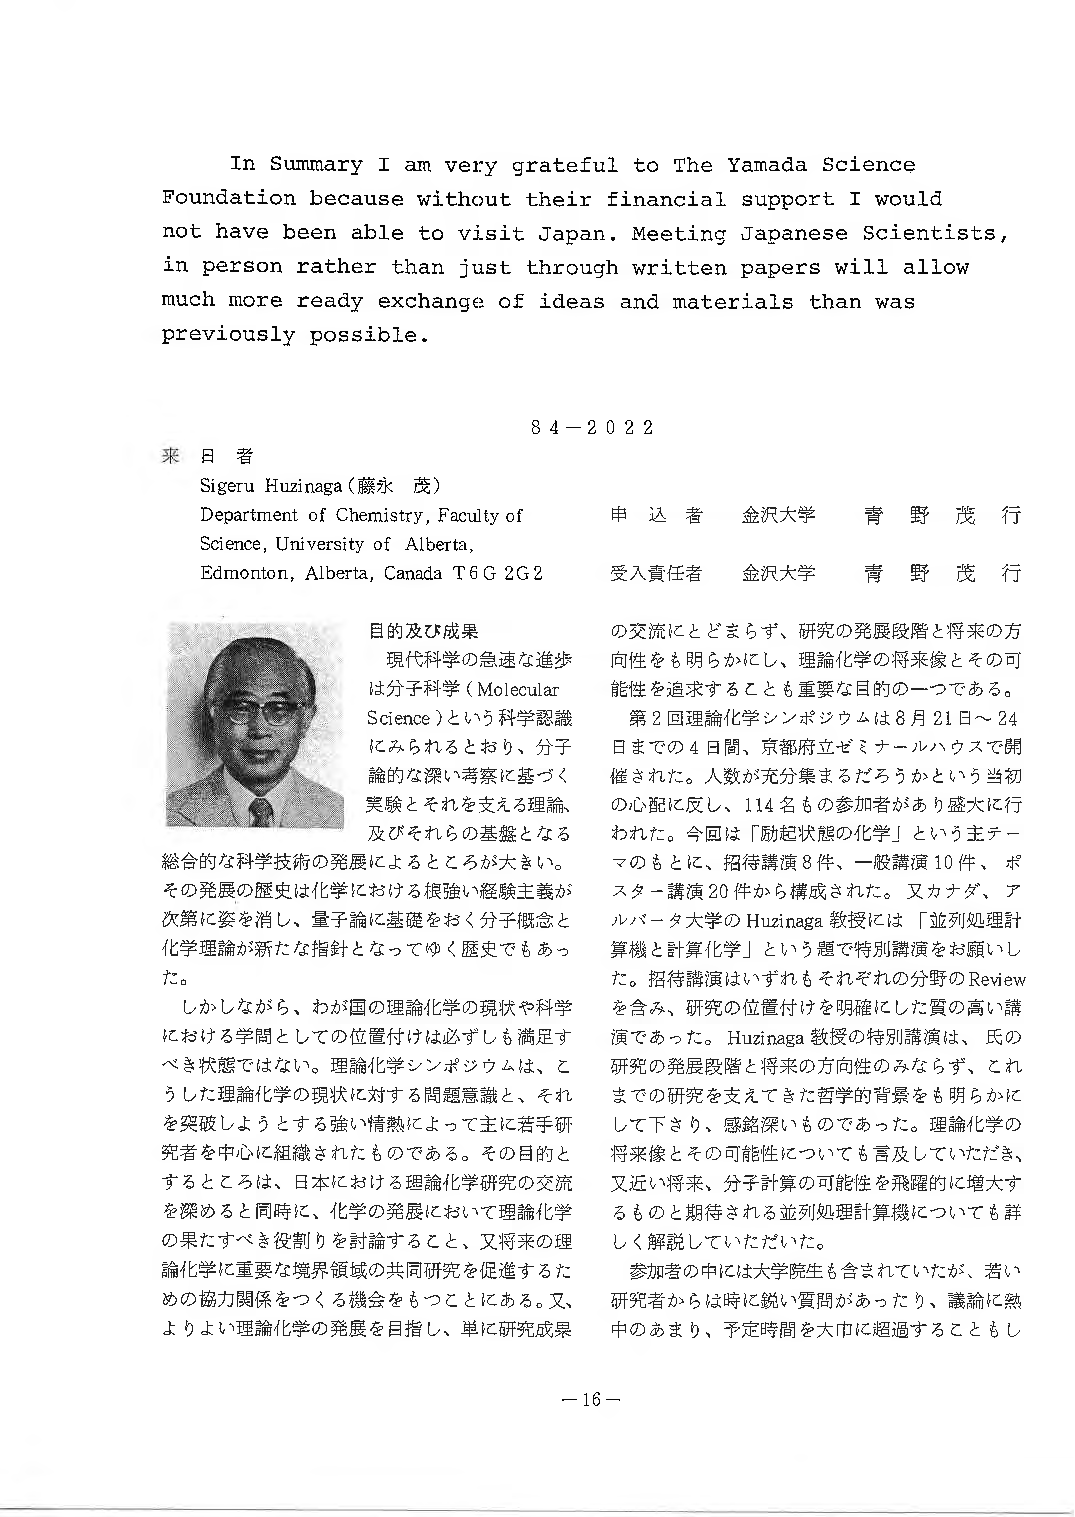
\includegraphics[width=\linewidth,height=27mm,keepaspectratio,
  trim=80bp 328bp 349bp 298bp,clip]{chapter-figures/portrait-huzinaga-source.pdf}}
{A Japanese quantum chemist and professor at the University of Alberta,
Huzinaga helped turn Gaussian basis functions into systematic tools for
molecular calculations. His 1965 atomic Gaussian expansions
\citep{Huzinaga1965} provided an influential foundation for practical basis
construction. His work connected the choice and contraction of atomic
functions with the accuracy and computational demands of molecular
electronic-structure calculations.}
{Biography: \href{https://www.registrar.ualberta.ca/calendar-archive/calendar-2015-2016/University-Staff/Emeriti/251.html}{University of Alberta emeriti record};
\href{https://www.molsci.jp/wp-content/uploads/A0002.pdf}{Huzinaga's account of computational chemistry, 2007}.
Portrait: \href{https://yamadazaidan.jp/wordpress/wp-content/uploads/2021/09/S60_Vol.1_18.pdf}{Yamada Science Foundation report, printed p.~16 (detail)};
photographer/date unspecified. \textbf{Draft reproduction: permission pending.}}}

\newcommand{\hfBioDunning}{%
\hfbiography{Thom H.~Dunning Jr. (b.~1943)}
{\hfbiophoto{chapter-figures/portrait-dunning.jpg}}
{An American theoretical chemist trained at Caltech, Dunning developed
Gaussian basis sets first for Hartree--Fock calculations and subsequently
for correlated wavefunctions. His correlation-consistent construction
\citep{Dunning1989} organizes basis functions into balanced hierarchical
sequences. This made systematic convergence toward the complete-basis limit
a practical strategy, linking basis design to the reliable assessment of
electronic-structure methods.}
{Biography and portrait: \href{https://www.iaqms.org/members/dunning.php}{IAQMS profile}.
Portrait photographer/date unspecified. \textbf{Draft reproduction: permission pending.}}}

\newcommand{\hfBioPauli}{%
\hfbiography{Wolfgang Pauli (1900--1958)}
{\hfbiophoto{chapter-figures/portrait-pauli.jpg}}
{Born in Vienna, Pauli became professor of theoretical physics at ETH
Z\"urich in 1928. His exclusion principle, proposed in 1925, was decisive
in understanding atomic electronic configurations \citep{Pauli1925} and
earned him the 1945 Nobel Prize in Physics. In the many-electron formulation
used here, exclusion follows from the antisymmetry of the electronic
wavefunction rather than from an additional rule imposed on its orbitals.}
{Biography: \href{https://archives.web.cern.ch/pauli_archive/biography/}{CERN Pauli Archive};
\href{https://www.nobelprize.org/prizes/physics/1945/pauli/facts/}{Nobel Foundation}.
Portrait: Bettina Katzenstein / ETH-Bibliothek Z\"urich, Bildarchiv,
\href{https://commons.wikimedia.org/wiki/File:Wolfgang_Pauli_ETH-Bib_Portr_01042_(cropped).jpg}{Portr 01042, crop by Xabier},
\href{https://creativecommons.org/licenses/by-sa/3.0/}{CC BY-SA 3.0}.}}

\newcommand{\hfBioSlater}{%
\hfbiography{John Clarke Slater (1900--1976)}
{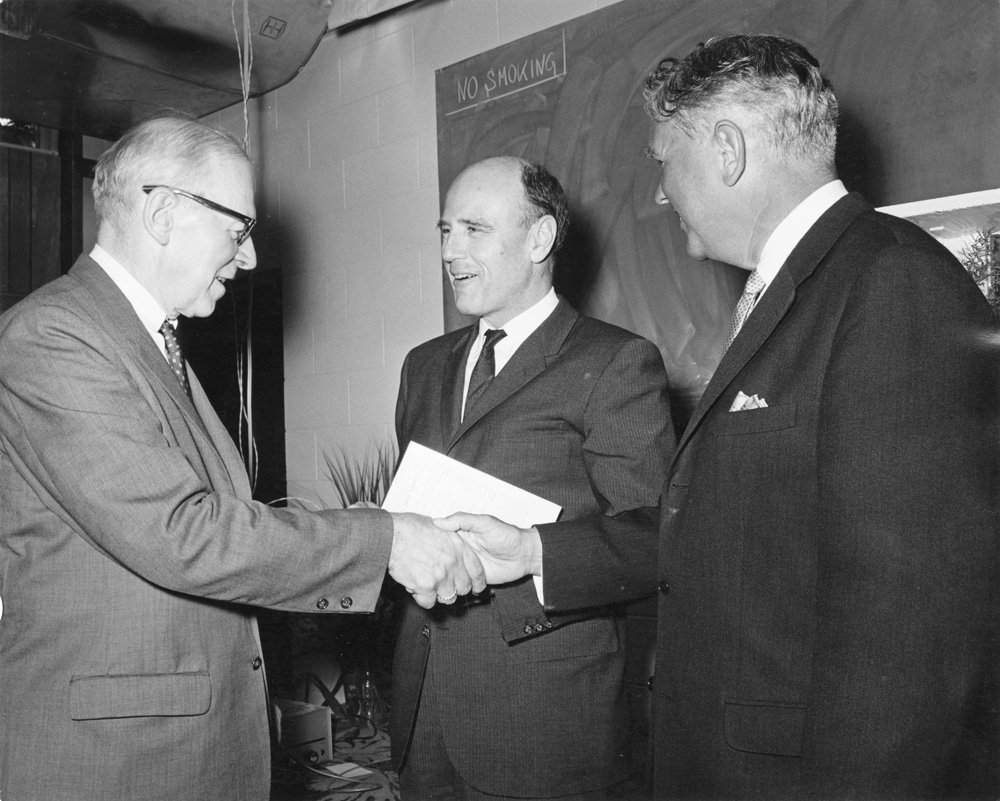
\includegraphics[width=\linewidth,height=27mm,keepaspectratio,
  trim=75bp 40bp 0bp 0bp,clip]{chapter-figures/slater-mulliken-1967.jpg}}
{An American physicist with a long career at MIT and later at the University
of Florida, Slater helped shape the quantum theory of atoms, molecules, and
solids. His 1929 determinantal wavefunctions provide the antisymmetric
building blocks used throughout this chapter \citep{Slater1929}.
His analytic atomic orbitals and screening rules also connect this
many-electron construction with the Slater-type basis functions introduced
in the second part \citep{Slater1930Orbitals}.}
{Biography: \href{https://www.nasonline.org/wp-content/uploads/2024/06/slater-john.pdf}{P.~M.~Morse, NAS memoir}.
Portrait detail: Larry C.~Huston, 1967; identified on the right in the
\href{https://photoarchive.lib.uchicago.edu/db.xqy?one=apf1-01019.xml}{archive description}.
University of Chicago Photographic Archive, apf1-01019, Hanna Holborn Gray Special Collections Research Center, University of Chicago Library.
\href{https://photoarchive.lib.uchicago.edu/rights.html}{Educational/scholarly reuse; commercial permission required}.}}

\newcommand{\hfBioCondon}{%
\hfbiography{Edward Uhler Condon (1902--1974)}
{\hfbiophoto{chapter-figures/portrait-condon.jpg}}
{Condon was an American theoretical physicist whose work connected the new
quantum mechanics with atomic and molecular spectroscopy. His treatment of
complex spectra contributed to the determinant matrix-element rules now
named after Slater and Condon \citep{Condon1930}. He worked at Princeton and
Westinghouse before directing the US National Bureau of Standards from 1945
to 1951, and later held academic appointments at Washington University and
the University of Colorado.}
{Biography: \href{https://history.aip.org/catalog/icos/1368.html}{American Institute of Physics, Condon papers};
\href{https://www.nist.gov/history/directors-national-bureau-standards-1901-1988-and-national-institute-standards-and}{NIST historical record}.
Portrait: National Bureau of Standards, 1947,
\href{https://commons.wikimedia.org/wiki/File:Edward_U._Condon_in_1947.jpg}{via Wikimedia Commons}; US federal-government photograph, public domain.}}

\newcommand{\hfBioBrillouin}{%
\hfbiography{L\'eon Nicolas Brillouin (1889--1969)}
{\hfbiophoto{chapter-figures/portrait-brillouin.jpg}}
{A French theoretical physicist, Brillouin held chairs in Paris before
continuing his career in the United States. His research encompassed wave
propagation, the electronic structure of solids, and the relation between
information and thermodynamics. His work on self-consistent fields led to
the stationarity result discussed here \citep{Brillouin1932}; his name is also
associated with Brillouin zones and the semiclassical WKB approximation.}
{Biography: \href{https://www.nasonline.org/wp-content/uploads/2024/06/brillouin-lon-n.pdf}{L.~Hilleth Thomas, NAS memoir}.
Portrait: Benjamin Couprie, Institut International de Physique Solvay,
\href{https://commons.wikimedia.org/wiki/File:L\%C3\%A9on_Brillouin_Solvay_conference_1927.jpg}{1927 Solvay photograph, crop by Setreset}; public domain.}}

\newcommand{\hfBioKoopmans}{%
\hfbiography{Tjalling Charles Koopmans (1910--1985)}
{\hfbiophoto{chapter-figures/portrait-koopmans.jpg}}
{Koopmans was born in the Netherlands and initially trained in mathematics
and physics. His 1934 paper related electron-removal energies to
Hartree--Fock orbital energies under the frozen-orbital approximation
\citep{Koopmans1934}. He subsequently turned to economics and joined Yale
in 1955. His later work on the allocation of resources brought him a share
of the 1975 Nobel Memorial Prize in Economic Sciences---an unusual career
link between electronic-structure theory and mathematical economics.}
{Biography: \href{https://cowles.yale.edu/people/tjalling-c-koopmans}{Yale University, Cowles Foundation}.
Portrait: Eric Koch / Anefo, Nationaal Archief,
\href{https://commons.wikimedia.org/wiki/File:TjallingKoopmans1967_(cropped).jpg}{Leuven, 1967, crop by Wabbuh},
\href{https://creativecommons.org/publicdomain/zero/1.0/}{CC0 1.0}.}}

\newcommand{\hfBioRoothaan}{%
\hfbiography{Clemens C.~J.~Roothaan (1918--2019)}
{\hfbiophoto{chapter-figures/portrait-roothaan.jpg}}
{Born in Nijmegen in the Netherlands, Roothaan earned his doctorate at the
University of Chicago under Robert Mulliken in 1950. His 1951 formulation
of the molecular self-consistent-field problem in a finite basis
\citep{Roothaan1951}, developed independently of Hall's, helped turn
Hartree--Fock theory into a practical computational method. He remained
closely involved in scientific computing, directing Chicago's Computation
Center from 1962 to 1968.}
{Biography: \href{https://emeritifaculty.uchicago.edu/news-announcements/article/clemens-c.j.-roothaan-1918-2019}{University of Chicago obituary}.
Portrait: University of Chicago Photographic Archive,
\href{https://photoarchive.lib.uchicago.edu/db.xqy?one=apf1-12856.xml}{apf1-12856}, Hanna Holborn Gray Special Collections Research Center, University of Chicago Library.
\href{https://photoarchive.lib.uchicago.edu/rights.html}{Educational/scholarly reuse; commercial permission required}.}}

\newcommand{\hfBioHall}{%
\hfbiography{George Garfield Hall (1925--2018)}
{\hfbiophoto{chapter-figures/portrait-hall.jpg}}
{Born in Belfast, Hall studied at Cambridge under John Lennard-Jones.
His 1951 treatment of molecular orbitals gave an independent derivation
of the matrix self-consistent-field equations now known as the
Roothaan--Hall equations \citep{Hall1951}. He became professor of applied
mathematics at Nottingham in 1962. Alongside quantum chemistry, his career
included substantial work in mathematical education, illustrating the
mathematical breadth behind the molecular-orbital methods.}
{Biography: \href{https://www.iaqms.org/obituary/GeorgeGarfieldHall.pdf}{IAQMS obituary}.
Portrait: \href{https://www.iaqms.org/deceased/hall.php}{IAQMS archive}; photographer and date unspecified.
\textbf{Draft reproduction: permission pending.}}}

\newcommand{\hfBioLowdin}{%
\hfbiography{Per-Olov L\"owdin (1916--2000)}
{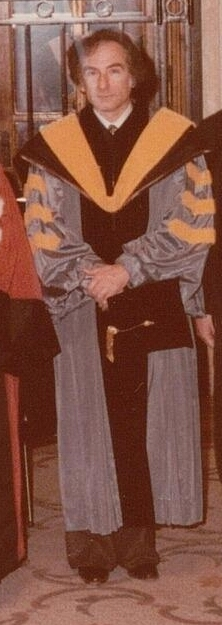
\includegraphics[width=\linewidth,height=27mm,keepaspectratio,
  trim=0bp 300bp 0bp 0bp,clip]{chapter-figures/portrait-lowdin.jpg}}
{A Swedish theoretical scientist, L\"owdin built influential quantum-chemistry
schools at Uppsala and the University of Florida. His 1950 study of
nonorthogonal atomic orbitals established the symmetric orthogonalization
used here \citep{Lowdin1950}. His research emphasized the mathematical
foundations of quantum chemistry, while his international summer and winter
schools and the Sanibel symposia helped train successive generations of
electronic-structure researchers.}
{Biography: \href{https://www.iaqms.org/deceased/lowdin.php}{IAQMS profile}.
Portrait: Sorbonne Universit\'e, unknown photographer, 25 November 1977,
\href{https://patrimoine.sorbonne-universite.fr/idurl/1/8392}{honorary-doctorate ceremony (detail)},
\href{https://www.etalab.gouv.fr/licence-ouverte-open-licence}{Licence Ouverte};
\href{https://commons.wikimedia.org/wiki/File:Per-Olov_L\%C3\%B6wdin.jpg}{via Wikimedia Commons}.}}

\newcommand{\hfBioBoys}{%
\hfbiography{Samuel Francis Boys (1911--1972)}
{\hfbiophoto{chapter-figures/portrait-boys.jpg}}
{A British theoretical chemist at Cambridge, Boys made Gaussian functions
central to practical molecular calculations through his 1950 work on
electronic wavefunctions \citep{Boys1950}. Efficient multicenter integrals
were a major part of their appeal. His later contributions included orbital
localization and, with Fernando Bernardi, the counterpoise correction for
basis-set superposition error \citep{FosterBoys1960,BoysBernardi1970}.
He was elected a Fellow of the Royal Society in 1972.}
{Biography: \href{https://www.iaqms.org/deceased/boys.php}{IAQMS profile};
\href{https://makingscience.royalsociety.org/people/na1119/samuel-francis-boys}{Royal Society record}.
Portrait: \href{https://www.iaqms.org/deceased/boys.php}{IAQMS archive}; photographer and date unspecified.
\textbf{Draft reproduction: permission pending.}}}
